\documentclass[uplatex]{jsarticle}
%数式
\usepackage{amsmath,amssymb,bm}
%箇条書き
\usepackage{enumerate}
%画像
\usepackage[dvipdfmx]{graphicx}

\pagestyle{empty}%ページ番号が欲しい場合は不要}

%−−−−−−−−−−−−−−以下変更不可−−−−−−−−−−−−−−−−−

\makeatletter

\def\department#1{\def\@department{#1}}
\def\id#1{\def\@id{#1}}

\def\@maketitle{
\begin{center}
  {\LARGE \@title \par}%タイトル
  \vskip 1em
  {\large \@date}%日付
  \vskip 0.5em
  {\large \@department}%科類
  \vskip 0.5em
  {\large \@id}%学籍番号
  \hspace{0.5em}
  {\large \@author}%著者
\end{center}
}

\makeatother

%−−−−−−−−−−−−−−以下変更可−−−−−−−−−−−−−−−−


%タイトルの表示設定

%{}内を書き換えてください。
\title{ディジタル回路の基礎}%タイトル
\date{\today}%日付 「\today」のままなら今日の日付が出力されます。
\department{工学部計数工学科 システム情報工学コース}%学部学科
\id{03-240641}%学籍番号
\author{山田哲士}%名前


%ここから文書
\begin{document}
\maketitle

\section{課題1}
\subsection{コード}
\begin{verbatim}
  module main (
    input sw0,
    input sw1,
    output led
  );

    assign led = sw0 & sw1;
    
  endmodule
\end{verbatim}

\subsection{実行結果}
\begin{figure}[hbtp]
  \centering
  \includegraphics[height=5cm]
    {./image/1.jpeg}
  \caption{and回路}
  \label{ラベル}
\end{figure}

\subsection{考察}
ちゃんとand回路が作成できていることが確認できた。

\section{課題2}
\subsection{コード}
\begin{verbatim}
  module full_adder (
    input xin,
    input yin,
    input cin,
    output sout,
    output cout
  );
      assign sout = (xin ^ yin) ^ cin;
    assign cout = (xin & yin) | ((xin ^ yin) & cin);
  endmodule  
\end{verbatim}

\subsection{実行結果}
\begin{figure}[hbtp]
  \centering
  \includegraphics[height=5cm]
    {./image/2-1.jpeg}
  \caption{合計1の場合}
  \label{ラベル}
\end{figure}
\clearpage
\begin{figure}[hbtp]
  \centering
  \includegraphics[height=5cm]
    {./image/2-2.jpeg}
  \caption{合計2の場合}
  \label{ラベル}
\end{figure}
\begin{figure}[hbtp]
  \centering
  \includegraphics[height=5cm]
    {./image/2-3.jpeg}
  \caption{合計3の場合}
  \label{ラベル}
\end{figure}

\subsection{考察}
全加算器が正常に動作していることが確認できた。

\section{課題3}
\subsection{コード}
\begin{verbatim}
  module rca_3bit (
    input x0,
    input x1,
    input x2,
    input y0,
    input y1,
    input y2,
    output s0,
    output s1,
    output s2,
    output cout
  );
      wire c0_out;
      wire c1_out;
      full_adder fa0(
      .xin(x0),
      .yin(y0),
      .cin(0),
      .sout(s0),
      .cout(c0_out)
      );
      full_adder fa1(
      .xin(x1),
      .yin(y1),
      .cin(c0_out),
      .sout(s1),
      .cout(c1_out)
      );
      full_adder fa2(
      .xin(x2),
      .yin(y2),
      .cin(c1_out),
      .sout(s2),
      .cout(cout)
      );
  
  endmodule
  
  module full_adder (
    input xin,
    input yin,
    input cin,
    output sout,
    output cout
  );
     assign sout = (xin ^ yin) ^ cin;
     assign cout = (xin & yin) | ((xin ^ yin) & cin);
  endmodule  
\end{verbatim}

\subsection{実行結果}
\begin{figure}[hbtp]
  \centering
  \includegraphics[height=5cm]
    {./image/3.jpeg}
  \caption{3bit加算器}
  \label{ラベル}
\end{figure}

\subsection{考察}
3bit加算器が正常に動作していることが確認できた。写真は$6+5=11$の場合である。

\section{課題4}
\subsection{コード}
\begin{verbatim}
  module multiplier_2bit(
    input x0,
    input x1,
    input y0,
    input y1,
    output s0,
    output s1,
    output s2,
    output cout
  );
      rca_3bit ans(
      .x0(x0 & y0),
      .x1(x1 & y0),
      .x2(0),
      .y0(0),
      .y1(x0 & y1),
      .y2(x1 & y1),
      .s0(s0),
      .s1(s1),
      .s2(s2),
      .cout(cout)
      );
      
  endmodule
  
  module rca_3bit (
    input x0,
    input x1,
    input x2,
    input y0,
    input y1,
    input y2,
    output s0,
    output s1,
    output s2,
    output cout
  );
      wire c0_out;
      wire c1_out;
      full_adder fa0(
      .xin(x0),
      .yin(y0),
      .cin(0),
      .sout(s0),
      .cout(c0_out)
      );
      full_adder fa1(
      .xin(x1),
      .yin(y1),
      .cin(c0_out),
      .sout(s1),
      .cout(c1_out)
      );
      full_adder fa2(
      .xin(x2),
      .yin(y2),
      .cin(c1_out),
      .sout(s2),
      .cout(cout)
      );
  
  endmodule
  
  module full_adder (
    input xin,
    input yin,
    input cin,
    output sout,
    output cout
  );
     assign sout = (xin ^ yin) ^ cin;
     assign cout = (xin & yin) | ((xin ^ yin) & cin);
  endmodule  
\end{verbatim}

\subsection{実行結果}
\begin{figure}[hbtp]
  \centering
  \includegraphics[height=5cm]
    {./image/4.jpeg}
  \caption{2bit乗算器}
  \label{ラベル}
\end{figure}

\subsection{考察}
2bit乗算器が正常に動作していることが確認できた。写真は$3*3=9$の場合である。

\section{課題5}
\subsection{コード}
\begin{verbatim}
  module seven_seg_decoder(
    input s0,
    input s1,
    input s2,
    input cout,
    output led_a,
    output led_b,
    output led_c,
    output led_d,
    output led_e,
    output led_f,
    output led_g
  );
      wire [2:0] s;
      assign s = {s2, s1, s0};
      reg [6:0] seg_pattern [0:7];
      
      initial begin
          seg_pattern[0] = 7'b1111110;
          seg_pattern[1] = 7'b0110000;
          seg_pattern[2] = 7'b1101101;
          seg_pattern[3] = 7'b1111001;
          seg_pattern[4] = 7'b0110011;
          seg_pattern[5] = 7'b1011011;
          seg_pattern[6] = 7'b1011111;
          seg_pattern[7] = 7'b1110000;
      end
      
      assign {led_a, led_b, led_c, led_d, led_e, led_f, led_g} = seg_pattern[s];
      
  endmodule
  
  
  
  module rca_3bit (
    input x0,
    input x1,
    input x2,
    input y0,
    input y1,
    input y2,
    output s0,
    output s1,
    output s2,
    output cout
  );
      wire c0_out;
      wire c1_out;
      full_adder fa0(
      .xin(x0),
      .yin(y0),
      .cin(0),
      .sout(s0),
      .cout(c0_out)
      );
      full_adder fa1(
      .xin(x1),
      .yin(y1),
      .cin(c0_out),
      .sout(s1),
      .cout(c1_out)
      );
      full_adder fa2(
      .xin(x2),
      .yin(y2),
      .cin(c1_out),
      .sout(s2),
      .cout(cout)
      );
  
  endmodule
  
  module full_adder (
    input xin,
    input yin,
    input cin,
    output sout,
    output cout
  );
     assign sout = (xin ^ yin) ^ cin;
     assign cout = (xin & yin) | ((xin ^ yin) & cin);
  endmodule  
\end{verbatim}

\subsection{実行結果}
\begin{figure}[hbtp]
  \centering
  \includegraphics[height=5cm]
    {./image/5-1.jpeg}
  \caption{1の場合}
  \label{ラベル}
\end{figure}
\begin{figure}[hbtp]
  \centering
  \includegraphics[height=5cm]
    {./image/5-2.jpeg}
  \caption{2の場合}
  \label{ラベル}
\end{figure}
\begin{figure}[hbtp]
  \centering
  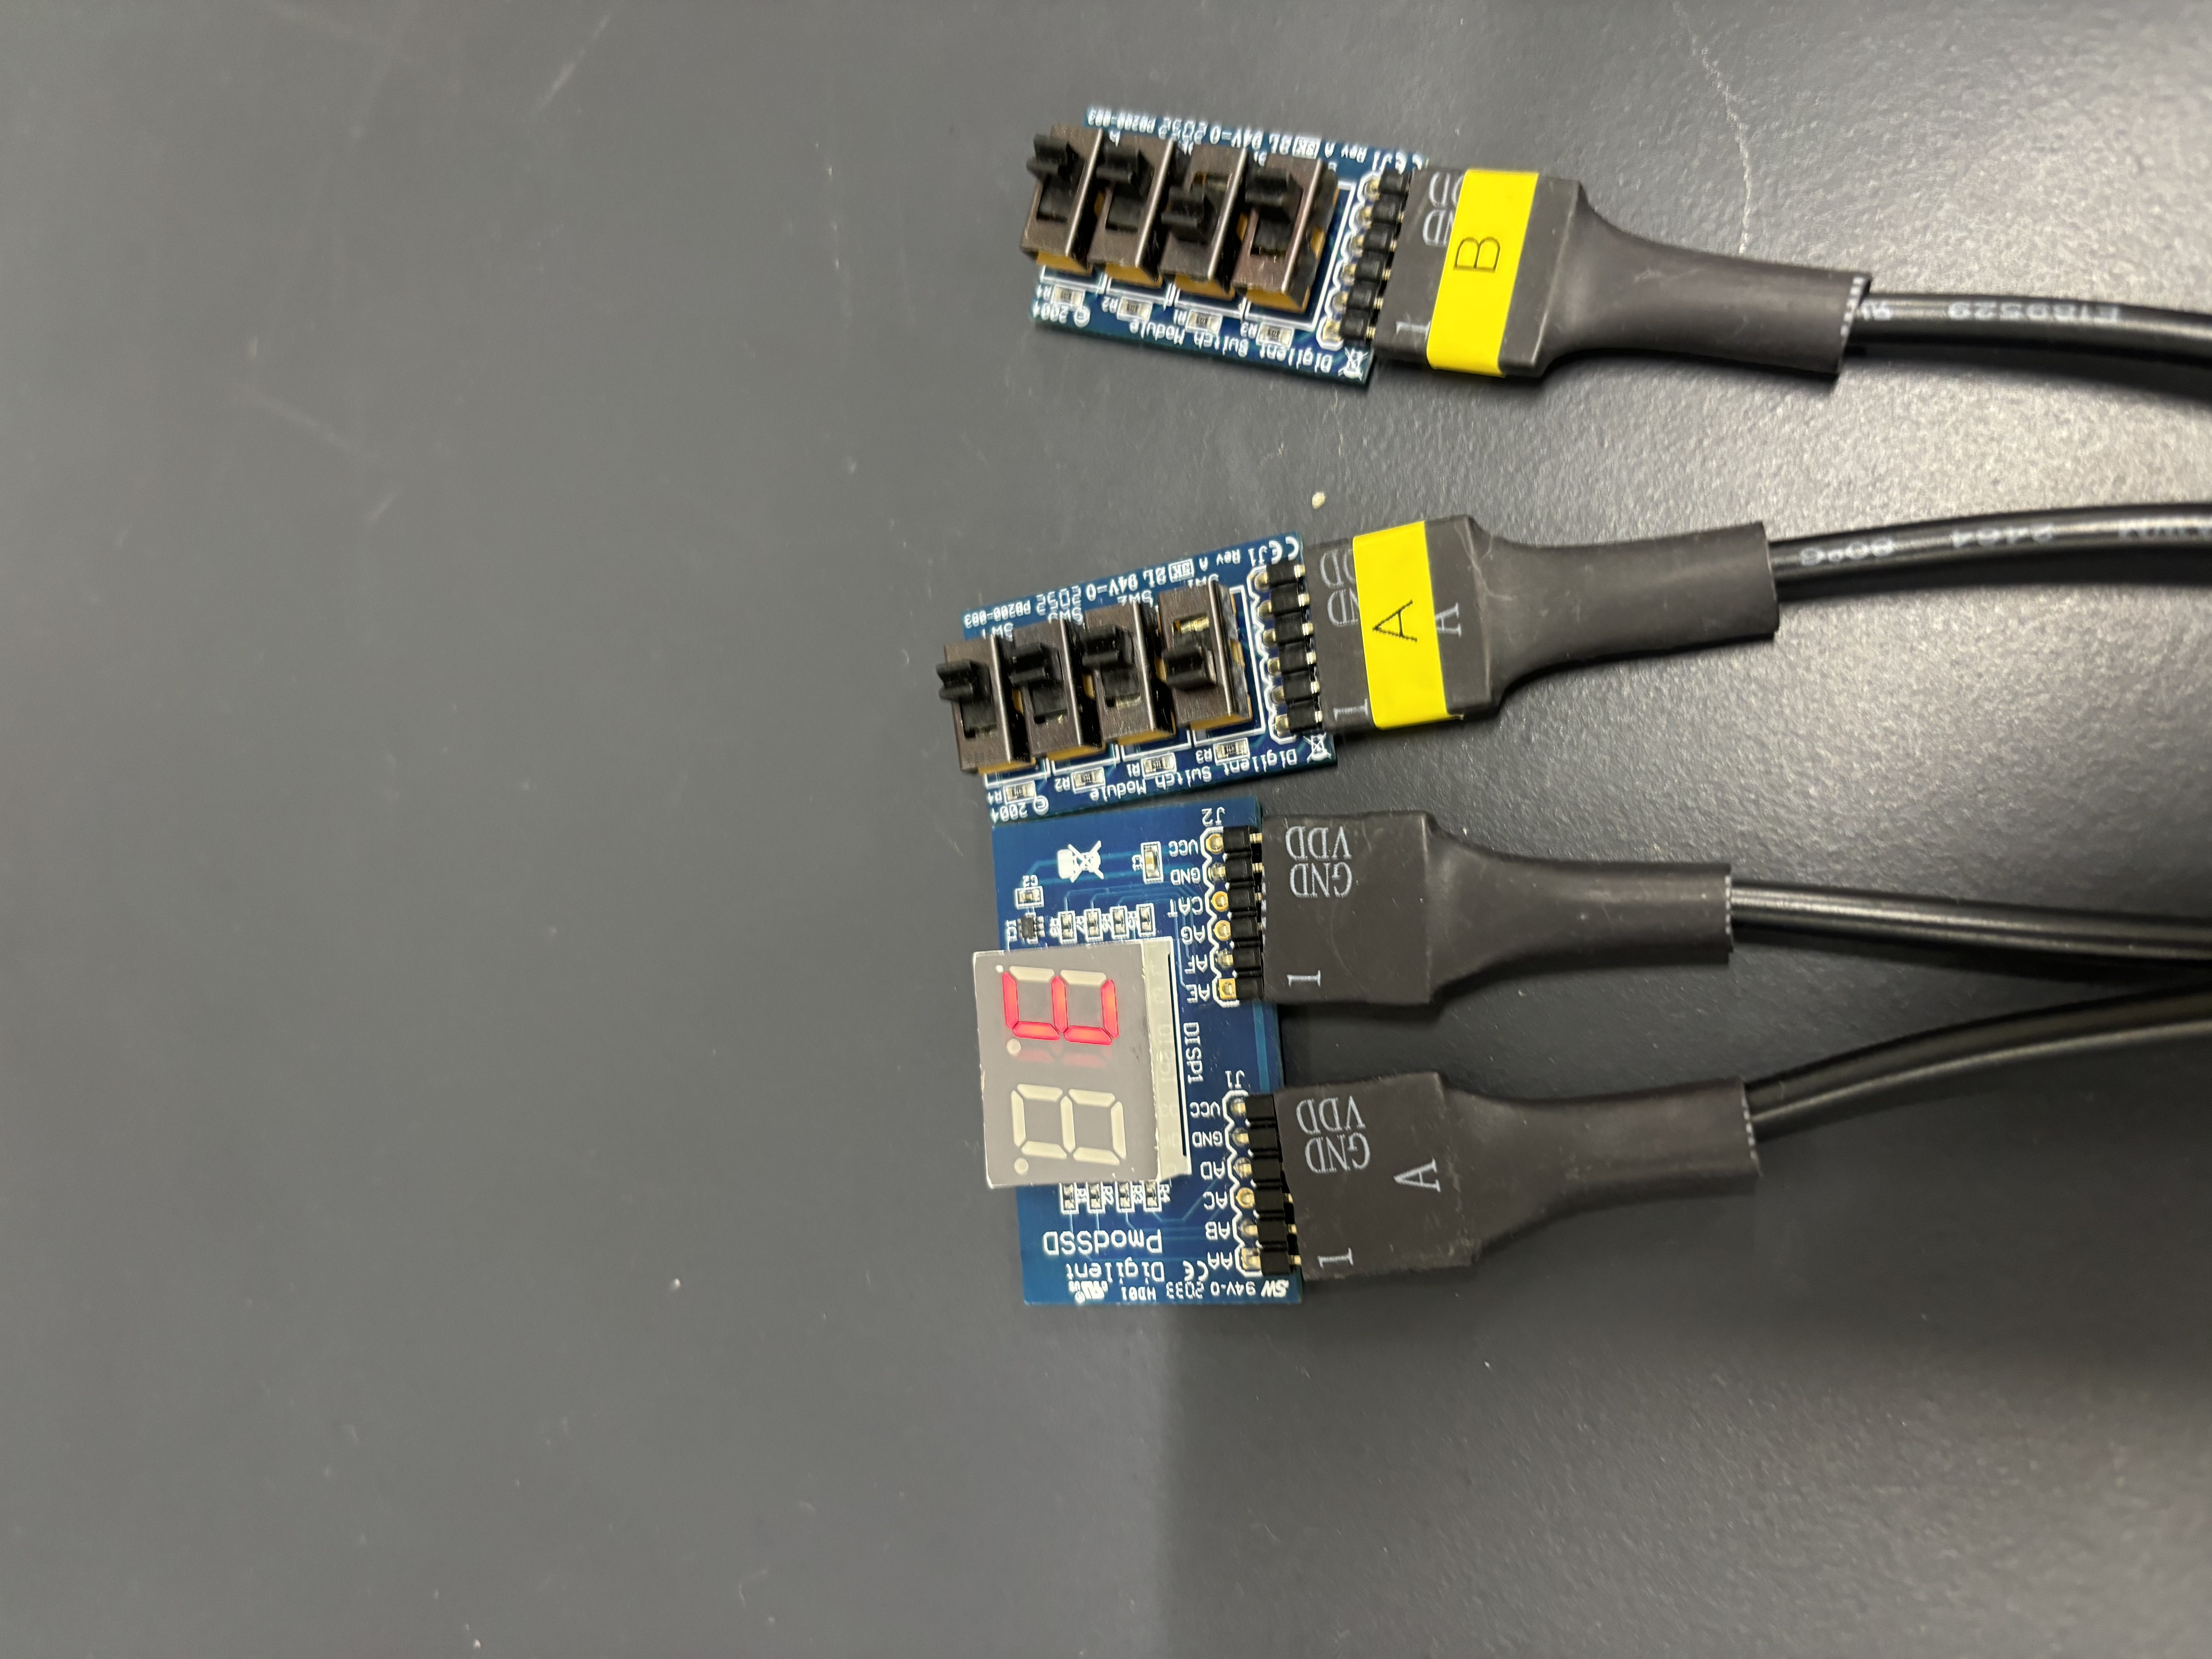
\includegraphics[height=5cm]
    {./image/5-3.jpeg}
  \caption{3の場合}
  \label{ラベル}
\end{figure}

\subsection{考察}
7セグメントデコーダが正常に動作していることが確認できた。写真は1,2,3の場合である。

\section{課題6}
\subsection{コード}
\begin{verbatim}
  `define COUNTER_W 4

  `define ENABLE 1'b1
  `define DISABLE 1'b0
  
  
  module counter_3bit(
    input clk,
    input reset_n,
    input enable,
    output reg[2:0] count
  );
       always @(posedge clk or negedge reset_n) begin
          if (!reset_n) begin
              count <= 3'b000;
          end else if (enable) begin
              count <= count + 1;
          end
      end
  
  endmodule
  
  module seven_seg_decoder(
    input [2:0] num,
    output led_a,
    output led_b,
    output led_c,
    output led_d,
    output led_e,
    output led_f,
    output led_g
  );
      reg [6:0] seg_pattern [0:7];
      
      initial begin
          seg_pattern[0] = 7'b1111110;
          seg_pattern[1] = 7'b0110000;
          seg_pattern[2] = 7'b1101101;
          seg_pattern[3] = 7'b1111001;
          seg_pattern[4] = 7'b0110011;
          seg_pattern[5] = 7'b1011011;
          seg_pattern[6] = 7'b1011111;
          seg_pattern[7] = 7'b1110000;
      end
      
      assign {led_a, led_b, led_c, led_d, led_e, led_f, led_g} = seg_pattern[num];
  
  endmodule
  
  
  module chattering_eliminator (
    input clk,
    input in_signal,
    output out_signal
  );
  
    reg [`COUNTER_W:0] r_count;
    reg r_out_signal;
    reg r_enable_delay;
    
  
    always @(posedge clk or negedge in_signal) begin
      if (!in_signal) begin
        r_count <= 0;
      end else begin
        if (!(&r_count == `ENABLE)) begin
          r_count <= r_count + 1;
        end
      end
    end
    
    always @(posedge clk) begin
       r_enable_delay <= &r_count;
    end
  
      assign out_signal = &r_count & !r_enable_delay;	
  
  endmodule  
\end{verbatim}

\subsection{実行結果}
以下のurlに動画を載せている。\\
\verb|https://drive.google.com/drive/folders/186rtjQShJ9BSqMBwmUW4zaLG3NnHokLI|

\subsection{考察}
カウンタが実装できていることが確認できた。また、チャタリング除去回路も正常に動作していることが確認できた。

\section{課題7}
\subsection{コード}
\begin{verbatim}
  `define COUNTER_W 4

  `define ENABLE 1'b1
  `define DISABLE 1'b0
  
  module state_machine (
    input clk,
    input reset_n,
    input btn0,
    input btn1,
    output reg state
  );
      reg current_state;
      
      parameter FIRST_PRESS = 1'b0;
      parameter SECOND_PRESS = 1'b1;
      parameter OFF = 1'b0;
      parameter ON = 1'b1;
      
      always @(posedge clk or negedge reset_n) begin
          if (!reset_n) begin
              current_state <= FIRST_PRESS;
              state <= OFF;
          end else begin
              case(current_state)
                  FIRST_PRESS: begin
                      if(btn0) begin
                          current_state <= SECOND_PRESS;
                          state <= OFF;
                      end else if(btn1) begin
                          current_state <= FIRST_PRESS;
                          state <= OFF;
                      end
                  end
                  SECOND_PRESS: begin
                      if(btn0) begin
                          current_state <= SECOND_PRESS;
                          state <= ON;
                      end else if (btn1) begin
                          current_state <= FIRST_PRESS;
                          state <= OFF;
                      end
                  end 
              endcase
          end
      end
     
  endmodule
  
  
  
  module chattering_eliminator (
    input clk,
    input in_signal,
    output out_signal
  );
  
    reg [`COUNTER_W:0] r_count;
    reg r_out_signal;
    reg r_enable_delay;
    
  
    always @(posedge clk or negedge in_signal) begin
      if (!in_signal) begin
        r_count <= 0;
      end else begin
        if (!(&r_count == `ENABLE)) begin
          r_count <= r_count + 1;
        end
      end
    end
    
    always @(posedge clk) begin
       r_enable_delay <= &r_count;
    end
  
      assign out_signal = &r_count & !r_enable_delay;	
  
  endmodule   
\end{verbatim}

\subsection{実行結果}
以下のurlに動画を載せている。\\
\verb|https://drive.google.com/drive/folders/186rtjQShJ9BSqMBwmUW4zaLG3NnHokLI|

\subsection{考察}
ステートマシンが正常に動作していることが確認できた。2回連続入力した時に状態が変わることが確認できた。また、3回連続入力した時も、2回でリセットするのではなく、光るように設定した。

\section{発展課題1}
\subsection{コード}
\begin{verbatim}
  module adder (
    input [15:0] a,
    input [15:0] b,
    output [15:0] s
  );
    wire [3:0] c; 

    cla_block block0(.a(a[3:0]), .b(b[3:0]), .cin(1'b0), .sum(s[3:0]), .cout(c[0])); 
    cla_block block1(.a(a[7:4]), .b(b[7:4]), .cin(c[0]), .sum(s[7:4]), .cout(c[1]));
    cla_block block2(.a(a[11:8]), .b(b[11:8]), .cin(c[1]), .sum(s[11:8]), .cout(c[2]));
    cla_block block3(.a(a[15:12]), .b(b[15:12]), .cin(c[2]), .sum(s[15:12]), .cout());
    
  endmodule


  module cla_unit (
      input a,
      input b,
      input cin,
      output p, 
      output g, 
      output sum
  );
      assign p = a ^ b;       
      assign g = a & b;       
      assign sum = p ^ cin;   
  endmodule

  module cla_block (
      input [3:0] a,
      input [3:0] b,
      input cin,
      output [3:0] sum,
      output cout,
      output g_out, 
      output p_out  
  );
      wire [3:0] p, g;
      wire [3:0] c; 

      cla_unit u0(.a(a[0]), .b(b[0]), .cin(cin), .p(p[0]), .g(g[0]), .sum(sum[0]));
      cla_unit u1(.a(a[1]), .b(b[1]), .cin(c[0]), .p(p[1]), .g(g[1]), .sum(sum[1]));
      cla_unit u2(.a(a[2]), .b(b[2]), .cin(c[1]), .p(p[2]), .g(g[2]), .sum(sum[2]));
      cla_unit u3(.a(a[3]), .b(b[3]), .cin(c[2]), .p(p[3]), .g(g[3]), .sum(sum[3]));

      assign c[0] = g[0] | (p[0] & cin);
      assign c[1] = g[1] | (p[1] & c[0]);
      assign c[2] = g[2] | (p[2] & c[1]);
      assign c[3] = g[3] | (p[3] & c[2]);
      assign cout = c[3];

      assign g_out = g[3] | (p[3] & g[2]) | (p[3] & p[2] & g[1]) | (p[3] & p[2] & p[1] & g[0]);
      assign p_out = p[3] & p[2] & p[1] & p[0];
  endmodule
\end{verbatim}

\subsection{実行結果}
\begin{figure}[hbtp]
  \centering
  \includegraphics[height=5cm]
    {./image/ad1.jpeg}
  \caption{16bit加算器}
  \label{ラベル}
\end{figure}

\subsection{考察}
16bit加算器が正常に動作していることが確認できた。また、このコードはキャリールックアヘッド加算器で実装している。ただ、時間がなく今回はリップルキャリー加算器の方は実装していない。

\end{document}